\documentclass[aspectratio=169, 10pt]{beamer}

\usepackage{bm} % bold math
\usepackage{fontspec}
\usepackage{minted}
\usepackage{pgf-pie}
\usepackage{tikz}

% Custom commands and environments
\makeatletter
\newcommand\version[1]{\renewcommand\@version{#1}}
\newcommand\@version{}
\def\insertversion{\@version}

\newcommand\course[1]{\renewcommand\@course{#1}}
\newcommand\@course{}
\def\insertcourse{\@course}

\newcommand\coursetitle[1]{\renewcommand\@coursetitle{#1}}
\newcommand\@coursetitle{}
\def\insertcoursetitle{\@coursetitle}

\newcommand\lecturenumber[1]{\renewcommand\@lecturenumber{#1}}
\newcommand\@lecturenumber{}
\def\insertlecturenumber{\@lecturenumber}
\makeatother

\newcommand{\slidetitle}[1]{{\xbseries \large \structure{#1}} \bigskip}
\newcommand{\term}[1]{{\color{blue} #1}}
\newcommand{\leftspace}{\hspace{1em}}
\newcommand{\inlinearrow}{
  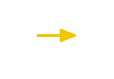
\begin{tikzpicture}[baseline]
    \node [anchor=base] (x) {};
    \draw [rawarrow] (x.mid west) -- ($(x.mid west) + (2em,0)$);
  \end{tikzpicture}
}

\newenvironment{slide}
{\begin{frame}[fragile,environment=slide]\vskip0pt plus 1filll}
{\vskip0pt plus 1filll\end{frame}}

% LaTeX

\setlength{\leftmargini}{1em}

% Common Information

\author{Jon Eyolfson}
\course{ECE 353}
\coursetitle{Systems Software}
\date{2024 Winter}

% fontspec

\defaultfontfeatures{Ligatures=TeX}
% \setmainfont{Domine}
\setsansfont{Inter}[
  FontFace={ul}{n}{Font=*-Thin},
  FontFace={el}{n}{Font=*-ExtraLight},
  FontFace={l}{n}{Font=*-Light},
  FontFace={sb}{n}{Font=*-SemiBold},
  FontFace={eb}{n}{Font=*-ExtraBold},
  FontFace={xb}{n}{Font=*-Black},
]
\setmonofont[Contextuals=AlternateOff, Ligatures=TeXOff]{Iosevka}[
  FontFace={xb}{n}{Font=*-Heavy},
]

%% Font Weights

\DeclareRobustCommand{\ulseries}{\fontseries{ul}\selectfont}
\DeclareTextFontCommand{\textul}{\ulseries}
\DeclareRobustCommand{\elseries}{\fontseries{el}\selectfont}
\DeclareTextFontCommand{\textel}{\elseries}
\DeclareRobustCommand{\lseries}{\fontseries{l}\selectfont}
\DeclareTextFontCommand{\textl}{\lseries}
\DeclareRobustCommand{\sbseries}{\fontseries{sb}\selectfont}
\DeclareTextFontCommand{\textsb}{\sbseries}
\DeclareRobustCommand{\ebseries}{\fontseries{eb}\selectfont}
\DeclareTextFontCommand{\texteb}{\ebseries}
\DeclareRobustCommand{\xbseries}{\fontseries{xb}\selectfont}
\DeclareTextFontCommand{\textxb}{\xbseries}

% tikz

\usetikzlibrary{
  arrows,
  arrows.meta,
  automata,
  backgrounds,
  calc,
  decorations.pathreplacing,
  matrix,
  positioning,
  overlay-beamer-styles,
  shapes,
  shapes.multipart,
  tikzmark,
}

\tikzstyle{rawarrow} = [
  -{Latex[round]},
  line width=1pt,
  yellow,
  shorten >=3pt,
  shorten <=3pt,
  font=\small,
  text=black,
]

\tikzstyle{arrow} = [
  -{Latex[round]},
  line width=1pt,
  yellow,
  shorten >=3pt,
  shorten <=3pt,
  transform canvas={yshift=3pt},
  font=\small,
  text=black,
]

\newcommand{\tikzmarkcoord}[1]{([yshift=3pt]pic cs:#1)}

% minted

\setminted{style=eyolfson, fontsize=\small, escapeinside=||}
\setmintedinline{fontsize=\normalsize}

% hyperref

\hypersetup{colorlinks, urlcolor=blue}

% beamer
\setbeamersize{text margin left=16mm, text margin right=16mm}
\setbeamertemplate{itemize items}[circle]
\setbeamercolor{item}{fg=black}
\setbeamercolor{structure}{fg=darkblue}
\setbeamerfont{frametitle}{series=\bfseries, parent=structure}
\setbeamertemplate{navigation symbols}{}
\setbeamertemplate{headline}{}
\setbeamertemplate{footline}{
  \begin{tikzpicture}[
    remember picture,
    overlay,
    shift={(current page.south west)},
  ]
    \path [fill=gray] (144mm, 0) -- (160mm, 16mm) -- (160mm, 0);
    \node [inner sep=3.5mm, outer sep=0, text=black, anchor=base east,
           align=right, yshift=3.5mm]
          at (current page.south east) {\ttfamily \small \insertframenumber{}};
  \end{tikzpicture}
}
\setbeamertemplate{title page}{
  \begin{tikzpicture}[
    remember picture,
    overlay,
    shift={(current page.south west)},
    background rectangle/.style={fill=darkblue},
    show background rectangle,
  ]
    \node [anchor=center, align=center, text=white, text width=40mm, scale=3.2]
          at (\paperwidth / 2, \paperheight * 2 / 3)
          {\xbseries \inserttitle{}};
    \node [anchor=base west, align=left, inner sep=0, text=white, yshift=2.5mm]
          at (16mm, \paperheight / 3)
          {\insertdate{} \insertcourse{}: \insertcoursetitle{}};
    \node [anchor=base west, align=left, inner sep=0, text=white, yshift=-2.5mm]
          at (16mm, \paperheight / 3)
          {\insertauthor};
    \node [anchor=base east, align=right, inner sep=0, text=white, yshift=2.5mm]
          at (144mm, \paperheight / 3)
          {Lecture \insertlecturenumber{}};
    \node [anchor=base east, align=right, inner sep=0, text=white,
           yshift=-2.5mm]
          at (144mm, \paperheight / 3)
          {\ttfamily \insertversion{}};
    \node [align=center, anchor=south, inner sep=0, text=white, yshift=3.5mm]
          (license) at (\paperwidth / 2, 0)
          {\fontsize{7pt}{7pt}\selectfont This  work is licensed under a
           \href{http://creativecommons.org/licenses/by-sa/4.0/}
                {\color{lightblue} Creative Commons Attribution-ShareAlike 4.0
                 International License}};
  \end{tikzpicture}
}

% xcolor

%% Primary Colour

\definecolor{pantone655}{RGB}{0, 42, 92} % #002a5c
\colorlet{darkblue}{pantone655}

%% Secondary Colours

\definecolor{pantone633}{RGB}{0, 139, 176} % #008bb0
\colorlet{blue}{pantone633}

\definecolor{pantonewarmred}{RGB}{220, 70, 51} % #dc4633
\colorlet{red}{pantonewarmred}

\definecolor{pantone3285}{RGB}{0, 161, 137} % #00a189
\colorlet{cyan}{pantone3285}

\definecolor{pantone7722}{RGB}{13, 83, 77} % #0d534d
\colorlet{darkcyan}{pantone7722}

\definecolor{pantone376}{RGB}{141, 191, 46} % #8dbf2e
\colorlet{green}{pantone376}

\definecolor{pantone2613}{RGB}{109, 36, 122} % #6d247a
\colorlet{violet}{pantone2613}

\definecolor{pantone2985}{RGB}{111, 199, 234} % #6fc7ea
\colorlet{lightblue}{pantone2985}

\definecolor{pantone227}{RGB}{171, 19, 104} % #ab1368
\colorlet{magenta}{pantone227}

\definecolor{pantone7406}{RGB}{241, 197, 0} % #f1c500
\colorlet{yellow}{pantone7406}

%% Neutrals

\definecolor{pantonecoolgray2}{RGB}{208, 209, 201} % #d0d1c9
\colorlet{gray}{pantonecoolgray2}


\lecturenumber{3}
\title{Libraries}
\version{2.0.0}

\begin{document}
  \begin{frame}[plain, noframenumbering]
    \titlepage
  \end{frame}

  \begin{slide}
    
    \slidetitle{What is an Operating System?}

    The kernel is part of an operating system, but what else?
    \bigskip

    Are macOS, iOS, iPadOS, watchOS, and tvOS all different operating systems?
  \end{slide}

  \begin{slide}
    \slidetitle{Applications May Pass Through Multiple Layers of Libraries}

    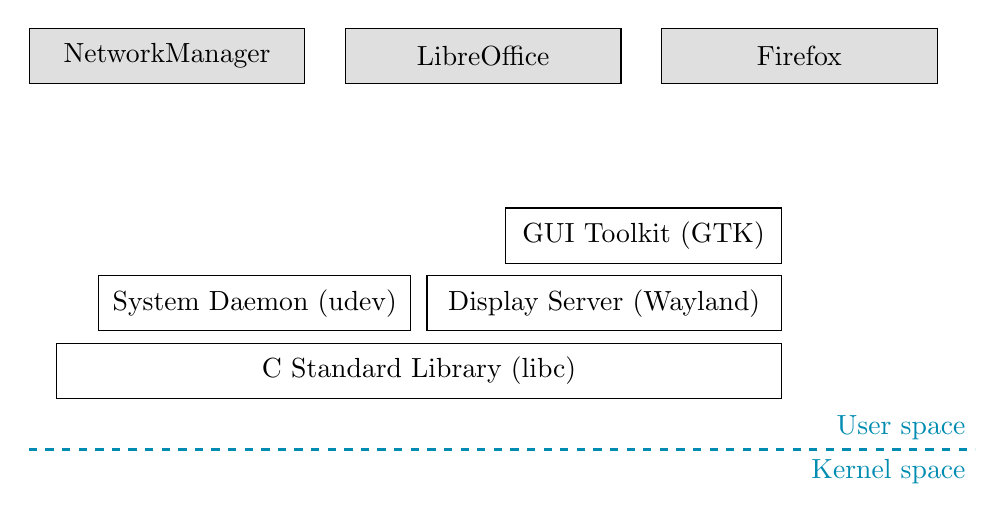
\begin{tikzpicture}[box/.style={draw, minimum width=3.5cm, minimum height=2em,
                                    inner sep=0.5em, node distance=0.5cm}]
      \draw [pantone633, dashed, thick] (0,0) -- ($(\textwidth - 3pt, 0)$);
      \node [pantone633, anchor=south east] at ($(\textwidth - 3pt, 0)$)
            (user) {User space};
      \node [pantone633, anchor=north east] at ($(\textwidth - 3pt, 0)$)
            (kernel) {Kernel space};

      \node [box, align=center, minimum width=9.2cm, xshift=-1cm] (libc) at ($(\textwidth/2 - 3pt, 1)$)
            {C Standard Library (libc)};

      \node [box, align=center, above=of libc, anchor=east, xshift=-0.1cm]
            {System Daemon (udev)};

      \node [box, align=center, above=of libc.north east, anchor=east, minimum width=4.5cm]
            (display) {Display Server (Wayland)};

      \node [box, above=of display.north east, anchor=east]
            {GUI Toolkit (GTK)};

      \node [box, fill=black!12.5,anchor=west] (app1) at (0, 5)
            {NetworkManager};

      \node [box, fill=black!12.5, right=of app1] (app2) {LibreOffice};

      \node [box, fill=black!12.5, right=of app2] {Firefox};
    \end{tikzpicture}
  \end{slide}

  \begin{slide}

    \slidetitle{What an Operating System is Depends on the Application}

    Android and Debian both use the Linux kernel,
    
    \leftspace{}but the applications are different
    \medskip

    Maybe they're the same OS if you only care about terminal applications
    \bigskip

    ``Linux'' distributions may be considered GNU/Linux

    \leftspace{}GNU distributes the standard C library and common utilities
    \bigskip

    An OS consists of a kernel and libraries required for your
    application
  \end{slide}

  \begin{slide}
    
    \slidetitle{Normal Compilation in C}

    \begin{center}
    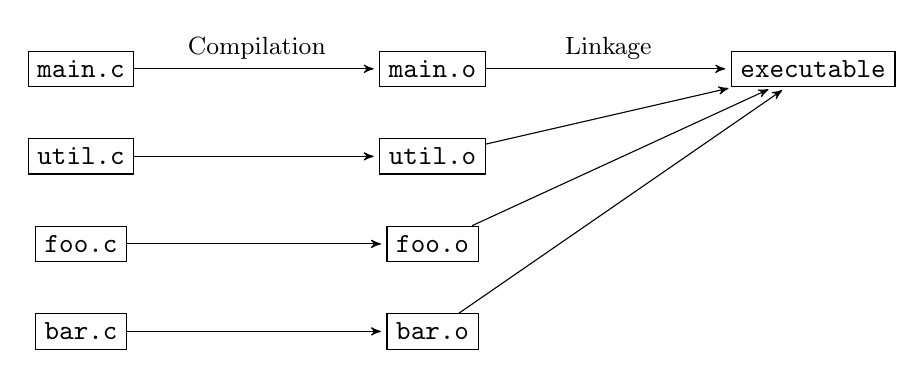
\begin{tikzpicture}[>=stealth', shorten >=2pt]
      \node[draw, align=left] (main) {\texttt{main.c}};
      \node[draw, align=left, below=of main, yshift=1em] (util)
           {\texttt{util.c}};
      \node[draw, align=left, below=of util, yshift=1em] (foo)
           {\texttt{foo.c}};
      \node[draw, align=left, below=of foo, yshift=1em] (bar)
           {\texttt{bar.c}};

      \node[draw, align=left, right=of main, xshift=6em] (main-obj)
           {\texttt{main.o}};
      \node[draw, align=left, below=of main-obj, yshift=1em] (util-obj)
           {\texttt{util.o}};
      \node[draw, align=left, below=of util-obj, yshift=1em] (foo-obj)
           {\texttt{foo.o}};
      \node[draw, align=left, below=of foo-obj, yshift=1em] (bar-obj)
           {\texttt{bar.o}};

      \node[draw, align=left, right=of main-obj, xshift=6em] (exec)
           {\texttt{executable}};

      \draw[->] (main) -- node [above] {\small Compilation} (main-obj);
      \draw[->] (util) -- (util-obj);
      \draw[->] (foo) -- (foo-obj);
      \draw[->] (bar) -- (bar-obj);
      \draw[->] (main-obj) -- node [above] {\small Linkage} (exec);
      \draw[->] (util-obj) -- (exec);
      \draw[->] (foo-obj) -- (exec);
      \draw[->] (bar-obj) -- (exec);
    \end{tikzpicture}
    \end{center}

    \vspace{1em}

    Note: object files (\texttt{.o}) are just ELF files with code for functions
  \end{slide}

  \begin{slide}
    
    \slidetitle{Static Libraries Are Included At Link Time}

    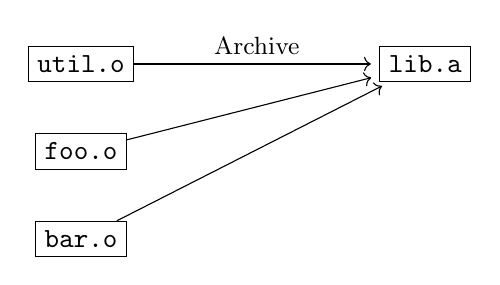
\begin{tikzpicture}[shorten >=3pt]
      \node[draw, align=left] (util-obj)
           {\texttt{util.o}};
      \node[draw, align=left, below=of util-obj, yshift=1em] (foo-obj)
           {\texttt{foo.o}};
      \node[draw, align=left, below=of foo-obj, yshift=1em] (bar-obj)
           {\texttt{bar.o}};

      \node[draw, align=left, right=of util-obj, xshift=6em] (static)
           {\texttt{lib.a}};

      \draw[->] (util-obj) -- node [above] {\small Archive} (static);
      \draw[->] (foo-obj) -- (static);
      \draw[->] (bar-obj) -- (static);
    \end{tikzpicture}

    \begin{flushright}
    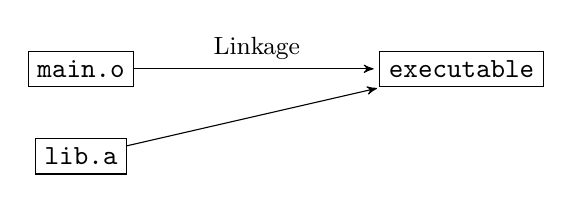
\begin{tikzpicture}[>=stealth', shorten >=2pt]

      \node[draw, align=left] (main-obj)
           {\texttt{main.o}};
      \node[draw, align=left, below=of main-obj, yshift=1em] (static)
           {\texttt{lib.a}};

      \node[draw, align=left, right=of main-obj, xshift=6em] (exec)
           {\texttt{executable}};

      \draw[->] (main-obj) -- node [above] {\small Linkage} (exec);
      \draw[->] (static) -- (exec);
    \end{tikzpicture}
    \end{flushright}
  \end{slide}

  \begin{slide}
    
    \slidetitle{Dynamic Libraries Are For Reusable Code}

    The C standard library is a dynamic library (\texttt{.so}), like any other
    on the system

    \leftspace{} Basically a collection of \texttt{.o} files containing function
    definitions
    \bigskip

    Multiple applications can use the same library:
    \medskip

    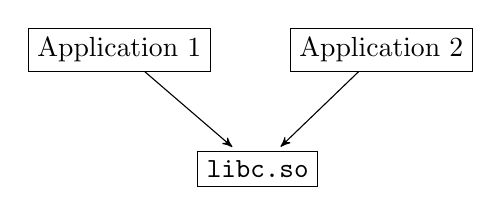
\begin{tikzpicture}[>=stealth', shorten >=2pt]
      \node[draw] (app1) {Application 1};
      \node[draw, right=of app1] (app2) {Application 2};
      \node[draw, below=of app1, xshift=5em] (libc) {\texttt{libc.so}};
      \draw[->] (app1) -- (libc);
      \draw[->] (app2) -- (libc);
    \end{tikzpicture}
    \medskip

    The operating system only loads \texttt{libc.so} in memory once, and shares
    it
  \end{slide}

  \begin{slide}
    
    \slidetitle{Dynamic Libraries Are Included At Runtime}

    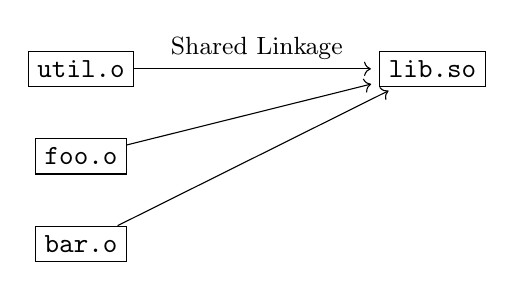
\begin{tikzpicture}[shorten >=3pt]
      \node[draw, align=left] (util-obj)
           {\texttt{util.o}};
      \node[draw, align=left, below=of util-obj, yshift=1em] (foo-obj)
           {\texttt{foo.o}};
      \node[draw, align=left, below=of foo-obj, yshift=1em] (bar-obj)
           {\texttt{bar.o}};

      \node[draw, align=left, right=of util-obj, xshift=6em] (static)
           {\texttt{lib.so}};

      \draw[->] (util-obj) -- node [above] {\small Shared Linkage} (static);
      \draw[->] (foo-obj) -- (static);
      \draw[->] (bar-obj) -- (static);
    \end{tikzpicture}

    \begin{flushright}
    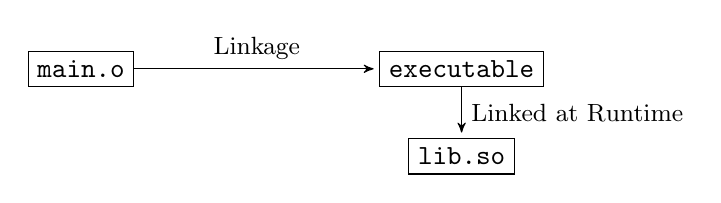
\begin{tikzpicture}[>=stealth', shorten >=2pt]

      \node[draw, align=left] (main-obj)
           {\texttt{main.o}};

      \node[draw, align=left, right=of main-obj, xshift=6em] (exec)
           {\texttt{executable}};

      \node[draw, align=left, below=of exec, yshift=1em] (dynamic)
           {\texttt{lib.so}};

      \draw[->] (main-obj) -- node [above] {\small Linkage} (exec);
      \draw[->] (exec) -- node [right] {\small Linked at Runtime} (dynamic);
    \end{tikzpicture}
    \end{flushright}
  \end{slide}

  \begin{slide}

    \slidetitle{Useful Command Line Utility for Dynamic Libraries}

    \texttt{ldd <executable>}
    
    \leftspace{}shows which dynamic libraries an executable uses
  \end{slide}

  \begin{slide}
    \slidetitle{Static vs Dynamic Libraries}

    Another option is to statically link your code

    \leftspace{}Basically copies the \texttt{.o} files directly into the
    executable
    \bigskip

    The drawbacks compared to dynamic libraries:
    \begin{itemize}
      \item Statically linking prevents re-using libraries
      
            (commonly used libraries have many duplicates)
      \item Any updates to a static library requires the executable to be
            recompiled
    \end{itemize}
    \bigskip

    What are issues with dynamic libraries?
  \end{slide}

  \begin{slide}
    \slidetitle{Dynamic Libraries Updates Can Break Executables}

    A dynamic library update may subtly change the ABI causing a crash
    \medskip

    Consider the following in a dynamic library:

    \leftspace{}A \texttt{struct} with multiple fields corresponding to
    a specific data layout (C ABI)
    \medskip

    \structure{An executable accesses the fields of the \texttt{struct} used by
               a dynamic library}
    \bigskip

    Now if a dynamic library reorders the fields

    \leftspace{} The executable uses the old offsets and is now wrong
    \medskip

    Note: this is OK if the dynamic library never exposes the fields of a
    \texttt{struct}
  \end{slide}

  \begin{slide}

    \slidetitle{
      C Uses a Consistent ABI for \texttt{\bfseries\color{magenta}struct}s
    }

    \texttt{struct}s are laid out in memory with the fields matching the
    declaration order

    \leftspace{}C compilers ensure the ABI of \texttt{struct}s are the
    consistent for an architecture
    \medskip

    Consider the following structures:
    \medskip
    \begin{columns}
      \begin{column}{0.4\textwidth}
        Library v1:
        \begin{minted}{c}
struct point {
  int y;
  int x;
};
        \end{minted}
      \end{column}
      \begin{column}{0.4\textwidth}
        Library v2:
        \begin{minted}{c}
struct point {
  int x;
  int y;
};
        \end{minted}
      \end{column}
    \end{columns}
    \medskip

    For v1 the \texttt{x} field is offset by 4 bytes from the start of
    \texttt{struct point}'s base

    \leftspace{}For v2 it is offset by 0 bytes, and this difference
    will cause problems
  \end{slide}

  \begin{slide}
    
    \slidetitle{After Compilation the Translation Differs for Each Version}
  
    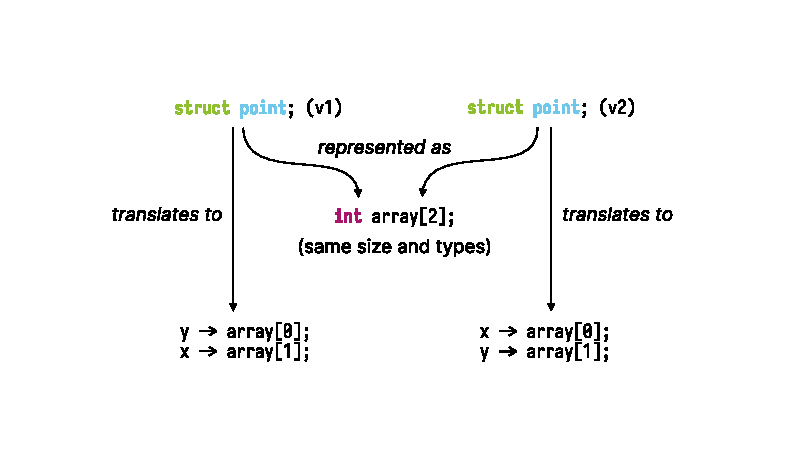
\includegraphics{point-representation.eps}

  \end{slide}

  \begin{slide}
    
    \slidetitle{The Point API Has Four Functions}

    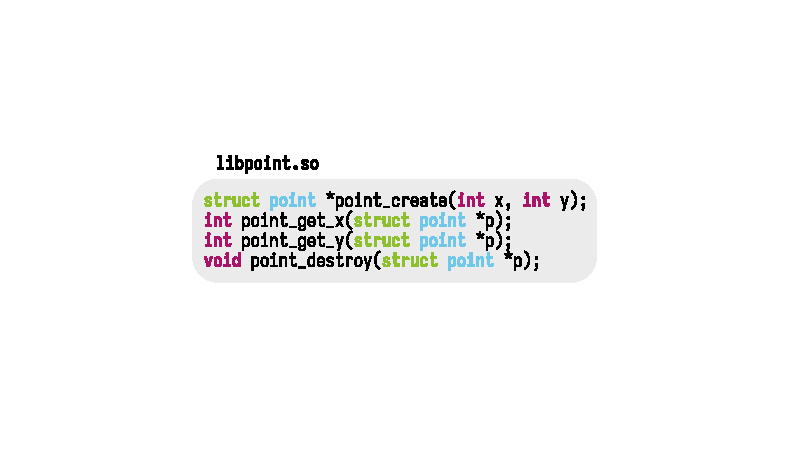
\includegraphics{point-api.eps}

  \end{slide}

  \begin{slide}

    \slidetitle{ABI Stable Code Should Always Print ``1, 2'' for Both Lines}
    
    \inputminted{c}{point-example.c}

  \end{slide}

  \begin{slide}

    \slidetitle{Try the Previous Example}

    We could set \texttt{LD\_LIBRARY\_PATH} to \mintinline{console}{build/v1} or \mintinline{console}{build/v2}
    to simulate a library update
    \bigskip

    Run the following commands to see for yourself:
    \begin{minted}{c}
build/point-example-compile-v1-link-v1
LD_LIBRARY_PATH=build/v2 build/point-example-compile-v1-link-v1
    \end{minted}
    \medskip

    Note: you'd also have a problem if you compiled with v2 and used v1
  \end{slide}

  \begin{slide}
    
    \slidetitle{Mismatched Versions Don't Agree on the Location of X and Y}
  
    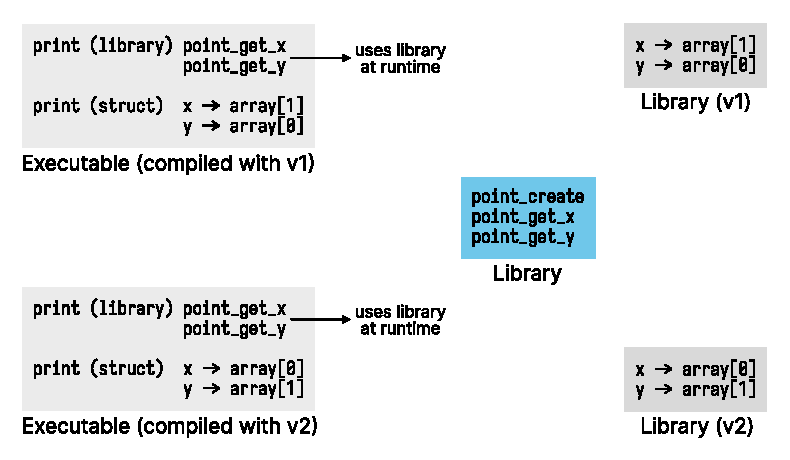
\includegraphics{point-libraries.eps}

  \end{slide}

  \begin{slide}

    \slidetitle{Mismatched Versions of This Library Causes Problems}

    The definition of \texttt{struct point} in both libraries is different

    \leftspace{}Order of \texttt{x} and \texttt{y} change (and therefore their
    offsets)
    \medskip

    Our code works correctly if the compiled and linked versions match

    \leftspace{}If you expose a \mintinline{c}{struct} it becomes part of your ABI!
    \bigskip

    Let's try executing different combinations:
    \begin{minted}{console}
build/point-example-compile-v1-link-v1
build/point-example-compile-v1-link-v2
build/point-example-compile-v2-link-v1
build/point-example-compile-v2-link-v2
    \end{minted}
    \medskip

    A proper stable ABI would hide the \mintinline{c}{struct} from
    \mintinline{c}{point.h}
  \end{slide}

  \begin{slide}

    \slidetitle{Semantic Versioning Meets Developer's Expectations}

    From \url{https://semver.org/}
    \medskip

    Given a version number MAJOR.MINOR.PATCH, increment the:
    \begin{itemize}
      \item MAJOR version when you make incompatible API\structure{/ABI} changes
      \item MINOR version when you add functionality in a backwards-compatible
            manner
      \item PATCH version when you make backwards-compatible bug fixes
    \end{itemize}
  \end{slide}

\begin{slide}
  
  \slidetitle{Dynamic Libraries Allow Easier Debugging}

  Control dynamic linking with environment variables

  \leftspace{}\texttt{LD\_LIBRARY\_PATH} and \texttt{LD\_PRELOAD}
  \medskip

  Consider the following example:

  \inputminted{c}{alloc-example.c}
\end{slide}

  \begin{slide}
    
    \slidetitle{We Can Monitor All Allocations with Our Own Library}

    Normal runs of \texttt{alloc-example} outputs:
    \begin{minted}{console}
x = 0x561116384260
    \end{minted}
    \medskip

    Create \texttt{liballoc-wrapper.so} that outputs all \texttt{malloc} and
    \texttt{free} calls \newline
    \leftspace{} Run: \mintinline{console}{LD_PRELOAD=build/liballoc-wrapper.so build/alloc-example}

    \begin{minted}{console}
Call to malloc(4) = 0x55c12aa40260                  
Call to malloc(1024) = 0x55c12aa40280
x = 0x55c12aa40260
Call to free(0x55c12aa40260)
    \end{minted}
    \bigskip

    Interesting, we did not make 2 \texttt{malloc} calls
  \end{slide}

\begin{slide}
  
  \slidetitle{Detecting Memory Leaks with Valgrind}

  \texttt{valgrind} is another useful tool to detect memory leaks from
  \texttt{malloc} and \texttt{free}

  \leftspace{}Usage: \texttt{valgrind <executable>}
  \bigskip


  Here's a note from the \texttt{man} pages regarding what we saw:
  \medskip

  ``The GNU C library (\texttt{libc.so}), which is used by all programs,
    may allocate memory for its own uses. Usually it doesn't bother to free
    that memory when the program ends—there would be no point, since the Linux
    kernel reclaims all process resources when a process exits anyway, so it
    would just slow things down.''
  \bigskip

  \structure{Note: this does not excuse you from not calling \texttt{free}!}
\end{slide}

\begin{slide}
  
  \slidetitle{Detecting Memory Leaks with AddressSanitizer}

  There's also sanitizer tools built into Clang (and now gcc), but you have to
  recompile

  \leftspace{}Add the \mintinline{console}{-Db_sanitize=address} flag to Meson
  \bigskip

  \begin{minted}{console}
rm -rf build
meson setup build -Db_sanitize=address
meson compile -C build
  \end{minted}
\end{slide}

\begin{slide}
  
  \slidetitle{System Calls are Rare in C}

  Mostly you'll be using functions from the C standard library instead
  \bigskip

  Most system calls have corresponding function calls in C, but may:
  \begin{itemize}
    \item Set \texttt{errno}
    \item Buffer reads and writes (reduce the number of system calls)
    \item Simplify interfaces (function combines two system calls)
    \item Add new features
  \end{itemize}
\end{slide}

\begin{slide}
  
  \slidetitle{C \texttt{exit} Has Additional Features}

  System call \texttt{exit} (or \texttt{exit\_group}): the program
  stops at that point
  \medskip

  C \texttt{exit}: there's a feature to register functions to call
  on program exit (\texttt{atexit})
  \medskip

  \inputminted{c}{atexit-example.c}
\end{slide}

\begin{slide}
  
  \slidetitle{Operating Systems Provide the Foundation for Libraries}

  We learned:
  \begin{itemize}
    \item Dynamic libraries and a comparison to static libraries
    \begin{itemize}
      \item How to manipulate the dynamic loader
    \end{itemize}
    \item Example of issues from ABI changes without API changes
  \end{itemize}

\end{slide}

\end{document}
